\newpage

\setcounter{section}{4}

\setcounter{subsection}{0}
\setcounter{figure}{0}
\setcounter{table}{0}

\renewcommand{\thesection}{\arabic{section}}

\counterwithin{subsection}{section}
\setcounter{subsection}{0}

\begin{center}
    \section*{\textbf{BAB IV \\ HASIL KEGIATAN}}
    \addcontentsline{toc}{section}{BAB IV \quad HASIL KEGIATAN}
\end{center}


\subsection{Hasil Kuantitatif}

Data kuantitatif dalam kegiatan ini diperoleh melalui penyebaran kuesioner kepada 177 responden yang berasal dari berbagai latar belakang usia, pekerjaan, dan agama. Data yang terkumpul kemudian dianalisis secara deskriptif untuk memperoleh gambaran mengenai pandangan responden terhadap hubungan antara nilai agama, moralitas, dan sikap antikorupsi. Analisis ini mencakup karakteristik responden, tingkat pengetahuan mengenai pandangan agama terhadap korupsi, serta persepsi responden terhadap peran agama dalam membentuk moral antikorupsi.   

Sebelum membahas hasil jawaban kuesioner, perlu diketahui terlebih dahulu karakteristik responden yang berpartisipasi dalam penelitian ini. Informasi mengenai latar belakang responden penting untuk memberikan gambaran mengenai keberagaman perspektif yang tercermin dalam hasil penelitian. Distribusi responden berdasarkan agama dan tingkat keaktifan dalam mengikuti kegiatan keagamaan disajikan pada Gambar 4.1. 

\begin{figure}[h]
            \centering
            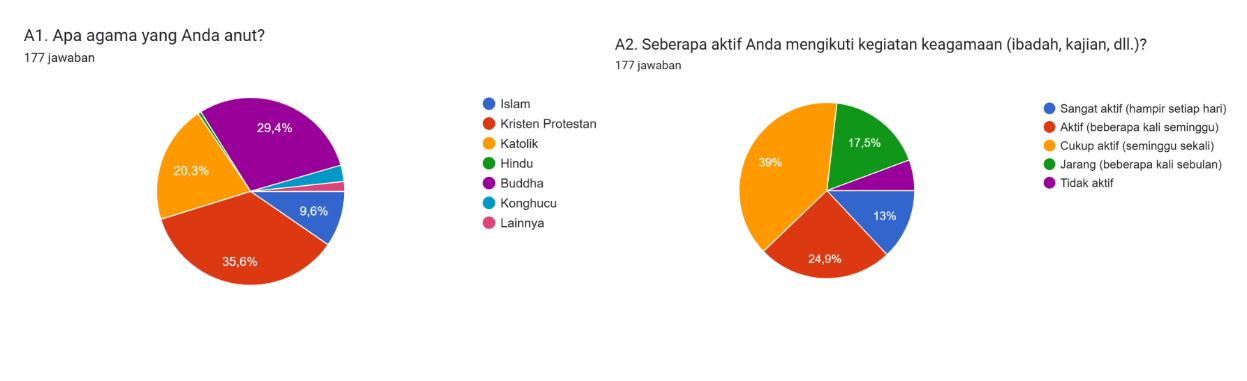
\includegraphics[width=\textwidth]{assets/respondent/distribusi_responden.png}
              \captionsetup{labelformat=empty}
               \caption[Diagram Distribusi Responden Berdasarkan Agama dan Keaktifan Kegiatan Keagamaan]{Gambar \ref{fig:PieChartpopulasi} Diagram distribusi responden berdasarkan agama dan keaktifan kegiatan keagamaan}
            \label{fig:PieChartpopulasi}
        \end{figure}

Berdasarkan Gambar 4.1, responden penelitian berasal dari latar belakang agama yang beragam. Mayoritas responden berasal dari agama Kristen Protestan sebesar 35,6%, diikuti oleh Buddha sebesar 29,4%, Katolik sebesar 20,3%, dan Islam sebesar 9,6%, sedangkan responden dari agama Hindu, Konghucu, dan agama lainnya memiliki persentase yang lebih kecil. Dari sisi keterlibatan dalam kegiatan keagamaan, mayoritas responden berada pada kategori cukup aktif sebesar 39%, diikuti kategori aktif sebesar 24,9%, jarang sebesar 17,5%, dan sangat aktif sebesar 13%.
        
Untuk memperoleh gambaran yang lebih jelas mengenai latar belakang agama responden, data distribusi responden berdasarkan agama disajikan pada Tabel 4.1.

\begin{table}[H]
\centering
\captionsetup{labelformat=empty}
\caption[Distribusi Responden Berdasarkan Agama]{Tabel \ref{tab:Tabelagama} Distribusi responden berdasarkan agama}
\label{tab:Tabelagama}
\begin{tabular}{ |c|c| } 
\hline
\textbf{Agama} & \textbf{Persentase (\%)} \\
\hline
Kristen Protestan & 35,6 \\ 
\hline
Buddha & 29,4 \\
\hline
Katolik & 20,3 \\
\hline
Islam & 9,6 \\
\hline
Hindu, Konghucu, dan lainnya & 5,1 \\
\hline
Total & 100\\
 
\hline
\end{tabular}
\end{table}

  
Berdasarkan Tabel 4.1, terlihat bahwa responden didominasi oleh penganut agama Kristen Protestan dan Buddha. Keberagaman latar belakang agama tersebut memungkinkan penelitian memperoleh pandangan yang lebih luas mengenai hubungan antara nilai keagamaan dan sikap terhadap korupsi.

Selain latar belakang agama, tingkat keaktifan responden dalam mengikuti kegiatan keagamaan juga menjadi salah satu aspek yang diamati dalam penelitian ini. Distribusi responden berdasarkan tingkat keaktifan kegiatan keagamaan disajikan pada Tabel 4.2. 

\begin{table}[H]
\centering
\captionsetup{labelformat=empty}
\caption[Distribusi responden berdasarkan keaktifan kegiatan keagamaan]{Tabel \ref{tab:Tabelkeaktifan} Distribusi responden berdasarkan keaktifan kegiatan keagamaan}
\label{tab:Tabelkeaktifan}
\begin{tabular}{ |c|c| } 
\hline
\textbf{Tingkat Keaktifan} & \textbf{Persentase (\%)} \\
\hline
Sangat aktif & 13 \\ 
\hline
Aktif & 24,9 \\
\hline
Cukup aktif & 39 \\
\hline
Jarang & 17,5 \\
\hline
Tidak aktif & 5,6 \\
\hline
Total & 100\\
\hline
\end{tabular}
\end{table}

Berdasarkan Tabel 4.2, sebagian besar responden berada pada kategori cukup aktif hingga aktif dalam mengikuti kegiatan keagamaan. Temuan ini menunjukkan bahwa mayoritas responden masih memiliki keterlibatan yang cukup rutin dalam aktivitas keagamaan, sehingga pandangan yang diberikan dalam kuesioner diharapkan cukup merepresentasikan pemahaman keagamaan yang dimiliki responden.

Setelah mengetahui karakteristik responden, analisis dilanjutkan pada hasil jawaban kuesioner yang berkaitan dengan pengetahuan dan pandangan responden mengenai korupsi dalam perspektif agama. Pertanyaan yang diberikan bertujuan untuk mengukur tingkat pemahaman responden mengenai larangan korupsi dalam agama, keberadaan sanksi moral atau spiritual bagi pelaku korupsi, serta paparan responden terhadap materi atau ceramah antikorupsi. 

Frekuensi jawaban responden pada pertanyaan pengetahuan dasar mengenai pandangan agama terhadap korupsi disajikan pada Tabel 4.3. 

\begin{table}[h]
\centering
\captionsetup{labelformat=empty}
\caption[Distribusi Jawaban Ya atau Tidak pada Pertanyaan Pengetahuan]{Tabel \ref{tab:Tabelpengetahuan} Distribusi jawaban ya atau tidak pada pertanyaan pengetahuan}
\label{tab:Tabelpengetahuan}
\begin{tabular}{ |c|p{8cm}|c|c| } 
\hline
\textbf{Kode} & \textbf{Pernyataan} & \textbf{Ya (\%)} & \textbf{Tidak (\%)} \\
\hline
B1 & Tahu agama melarang korupsi secara eksplisit & 95,5 & 4,5 \\ 
\hline
B2 & Pernah mendengar ceramah antikorupsi & 81,4 & 18,6 \\
\hline
B3 & Tahu adanya sanksi moral atau spiritual untuk pelaku korupsi & 94,4 & 5,6 \\
\hline
\end{tabular}
\end{table}

Data pada Tabel 4.3 menunjukkan bahwa mayoritas responden mengetahui bahwa agama mereka secara eksplisit melarang tindakan korupsi. Sebagian besar responden juga memahami adanya konsekuensi moral maupun spiritual yang dapat diterima oleh pelaku korupsi. Namun demikian, masih terdapat sejumlah responden yang belum pernah memperoleh ceramah atau pembinaan khusus mengenai antikorupsi. Temuan ini menunjukkan bahwa pemahaman dasar mengenai larangan korupsi dalam agama sudah cukup tinggi, tetapi upaya penyampaian nilai-nilai antikorupsi melalui kegiatan keagamaan masih dapat ditingkatkan.

Untuk memperoleh gambaran yang lebih mendalam mengenai sikap responden terhadap nilai agama dan perilaku antikorupsi, digunakan pertanyaan dengan skala Likert. Hasil rata-rata jawaban responden terhadap setiap pernyataan disajikan pada Tabel 4.4. 

\begin{table}[H]
    \centering
    \captionsetup{labelformat=empty}
    \caption[Skor rata-rata skala Likert sikap antikorupsi]{Tabel \ref{tab:Tabelhasilkuesioner} Skor rata-rata skala Likert sikap antikorupsi}
    \label{tab:Tabelhasilkuesioner}
    \begin{tabular}{ |c|p{8cm}|c|c| } 
    \hline
    \textbf{Kode} & \textbf{Pernyataan} & \textbf{Rata-Rata} & \textbf{Interpretasi} \\
    \hline
    B4 & Korupsi bertentangan dengan nilai-nilai agama saya & 4,62 & Sangat Setuju \\
    \hline
    B5 & Saya mengetahui tokoh agama yang aktif kampanye antikorupsi & 3,67 & Setuju \\
    \hline
    B6 & Ajaran agama telah memberikan pedoman yang jelas mengenai cara bekerja secara halal dan jujur & 4,56 & Sangat Setuju \\
    \hline
    C1 & Keyakinan agama menjadi alasan kuat menolak korupsi & 4,19 & Setuju \\
    \hline
    C2 & Saya merasa bertanggung jawab moral jika membiarkan korupsi & 3,93 & Setuju \\
    \hline
    C3 & Lembaga keagamaan berperan penting membangun budaya antikorupsi & 4,18 & Setuju \\
    \hline
    C4 & Orang taat beragama seharusnya tidak korupsi & 3,80 & Setuju \\
    \hline
    C5 & Ceramah antikorupsi berdampak nyata pada perilaku saya & 3,88 & Setuju \\
    \hline
    C6 & Rasa malu dan takut akibat spiritual mendorong saya jujur & 4,34 & Sangat Setuju \\
    \hline
    C7 & Pendidikan agama sejak kecil membentuk karakter antikorupsi & 4,27 & Setuju \\
    \hline
    C8 & Korupsi pasti membawa konsekuensi spiritual bagi pelakunya & 4,48 & Sangat Setuju \\
    \hline
    \end{tabular}
\end{table}

Berdasarkan Tabel 4.4, skor tertinggi diperoleh pada pernyataan bahwa korupsi bertentangan dengan nilai-nilai agama responden dengan nilai rata-rata sebesar 4,62. Pernyataan mengenai ajaran agama yang memberikan pedoman untuk bekerja secara halal dan jujur juga memperoleh skor yang tinggi, yaitu sebesar 4,56. Temuan ini menunjukkan bahwa responden memiliki keyakinan yang kuat bahwa agama mengajarkan nilai kejujuran dan menolak tindakan korupsi. 

Di sisi lain, skor yang relatif lebih rendah ditemukan pada pernyataan mengenai keberadaan tokoh agama yang aktif mengampanyekan antikorupsi dengan nilai rata-rata 3,67 serta dampak ceramah antikorupsi terhadap perilaku dengan nilai rata-rata 3,88. Hasil tersebut mengindikasikan bahwa meskipun pemahaman keagamaan mengenai korupsi sudah cukup baik, peran keteladanan tokoh agama dan efektivitas penyampaian pesan antikorupsi masih perlu diperkuat agar nilai-nilai agama dapat lebih nyata memengaruhi perilaku masyarakat. 

\subsection{Hasil Kualitatif}

Data kualitatif dalam penelitian ini diperoleh melalui wawancara dengan lima tokoh agama yang mewakili agama Buddha, Kristen, Katolik, Hindu, dan Islam. Wawancara dilakukan untuk memperoleh pemahaman yang lebih mendalam mengenai pandangan masing-masing agama terhadap tindakan korupsi, faktor-faktor yang menyebabkan praktik korupsi tetap terjadi di tengah masyarakat yang religius, serta peran agama dalam membentuk karakter dan moral antikorupsi. Hasil wawancara menunjukkan bahwa meskipun setiap agama memiliki ajaran dan pendekatan yang berbeda, seluruh narasumber sepakat bahwa korupsi merupakan tindakan yang bertentangan dengan nilai-nilai moral dan keagamaan. 

Narasumber dari agama Buddha menjelaskan bahwa korupsi merupakan pelanggaran terhadap Sila Kedua dalam Pancasila Buddhis, yaitu larangan mengambil sesuatu yang tidak diberikan atau bukan haknya. Tindakan korupsi dipandang berakar pada keserakahan dan kebodohan batin yang mendorong seseorang untuk mengabaikan nilai-nilai moral. Oleh karena itu, pencegahan korupsi perlu dilakukan melalui pengendalian diri, pengembangan rasa cukup, serta penerapan prinsip mata pencaharian benar dalam kehidupan sehari-hari. 

Pandangan yang serupa juga ditemukan dalam agama Kristen. Korupsi dipahami sebagai bentuk dosa karena berkaitan dengan tindakan mencuri dan kecintaan yang berlebihan terhadap uang. Menurut narasumber, umat Kristen perlu membangun sikap syukur, kejujuran, dan tanggung jawab dalam pekerjaan maupun kehidupan sosial. Selain itu, konsep menjadi “garam dan terang dunia” mengajarkan bahwa seseorang tidak hanya dituntut untuk menjauhi korupsi, tetapi juga menjadi teladan yang memberikan pengaruh positif bagi lingkungan sekitarnya. 

Sementara itu, narasumber dari agama Katolik menekankan bahwa korupsi tidak hanya merupakan kesalahan individu, tetapi juga termasuk dosa sosial karena dampaknya merugikan banyak orang dan menghambat terwujudnya kesejahteraan bersama. Oleh sebab itu, penghayatan iman tidak boleh berhenti pada praktik ritual keagamaan semata, melainkan perlu diwujudkan dalam kehidupan sosial melalui keberanian menolak gratifikasi, membiasakan perilaku jujur, dan mengutamakan kepentingan bersama di atas kepentingan pribadi. 

Dalam ajaran Hindu, korupsi dipahami sebagai tindakan yang bertentangan dengan Dharma karena melibatkan pengambilan hak yang bukan miliknya. Narasumber menjelaskan bahwa pencarian harta atau Artha harus selalu dilandasi oleh Dharma agar tidak berubah menjadi keserakahan yang merugikan orang lain. Selain itu, nilai Tri Kaya Parisudha yang menekankan kesucian pikiran, perkataan, dan perbuatan menjadi pedoman penting dalam membentuk perilaku yang jujur dan bertanggung jawab. 

\subsection{Pembahasan}
Hasil wawancara dan kuesioner menunjukkan adanya pola yang konsisten, yaitu seluruh agama memiliki landasan moral yang kuat dalam menolak tindakan korupsi. Korupsi dipahami sebagai tindakan mengambil hak orang lain secara tidak sah, baik dalam bentuk uang, waktu, jabatan, maupun kewenangan. Pandangan ini muncul dalam wawancara dengan tokoh agama Buddha, Kristen, Katolik, Hindu, dan Islam. Dengan demikian, secara normatif agama memiliki posisi yang jelas dalam menolak korupsi.

Meskipun demikian, hasil penelitian menunjukkan adanya kesenjangan antara pengetahuan agama dan penerapan moral dalam kehidupan nyata. Hal ini terlihat dari tingginya persentase responden yang mengetahui bahwa agama melarang korupsi, tetapi skor mengenai dampak ceramah antikorupsi terhadap perilaku masih lebih rendah dibandingkan skor keyakinan teologis. Kondisi ini menunjukkan bahwa masyarakat tidak hanya membutuhkan pengetahuan bahwa korupsi itu salah, tetapi juga membutuhkan pembinaan moral yang mampu menjawab situasi konkret dalam kehidupan sehari-hari.

Kesenjangan tersebut juga terlihat dari rendahnya skor mengenai pengetahuan responden terhadap tokoh agama yang aktif mengampanyekan antikorupsi. Artinya, masyarakat belum cukup terekspos pada figur keteladanan yang secara nyata menyuarakan nilai antikorupsi di ruang publik. Padahal, tokoh agama memiliki peran penting sebagai panutan moral yang dapat membantu masyarakat menerjemahkan ajaran agama menjadi tindakan nyata.

Berdasarkan hasil tersebut, penanaman moral antikorupsi tidak cukup dilakukan melalui ceramah yang hanya bersifat normatif. Pembinaan keagamaan perlu dikembangkan menjadi diskusi moral yang lebih kontekstual, misalnya dengan membahas kasus suap, gratifikasi, manipulasi data, titip absen, plagiarisme, dan bentuk ketidakjujuran lain yang dekat dengan kehidupan masyarakat. Dengan demikian, nilai agama tidak hanya dipahami sebagai aturan, tetapi juga menjadi dasar dalam mengambil keputusan moral.

\newpage

Selain itu, pendidikan antikorupsi berbasis nilai agama perlu diterapkan sejak dini melalui keluarga, sekolah, lembaga keagamaan, dan masyarakat. Keluarga dapat membiasakan kejujuran dalam kehidupan sehari-hari, sekolah dapat menanamkan integritas melalui aturan dan pembelajaran, sedangkan lembaga keagamaan dapat memperkuat kesadaran moral melalui pembinaan yang relevan dengan realitas sosial. Kolaborasi berbagai pihak tersebut diperlukan agar nilai kejujuran, tanggung jawab, dan integritas dapat benar-benar diterapkan dalam kehidupan masyarakat.

\subsection{Dokumentasi Kegiatan}

Dokumentasi kegiatan disajikan sebagai pelengkap laporan untuk memberikan gambaran mengenai pelaksanaan kegiatan yang telah dilakukan. Dokumentasi ini menunjukkan keterlibatan para narasumber dalam proses pengumpulan data serta menjadi bukti pelaksanaan kegiatan yang mendukung penyusunan laporan. Salah satu dokumentasi kegiatan dapat dilihat pada Gambar 4.2.

\begin{figure}[H]
            \centering
            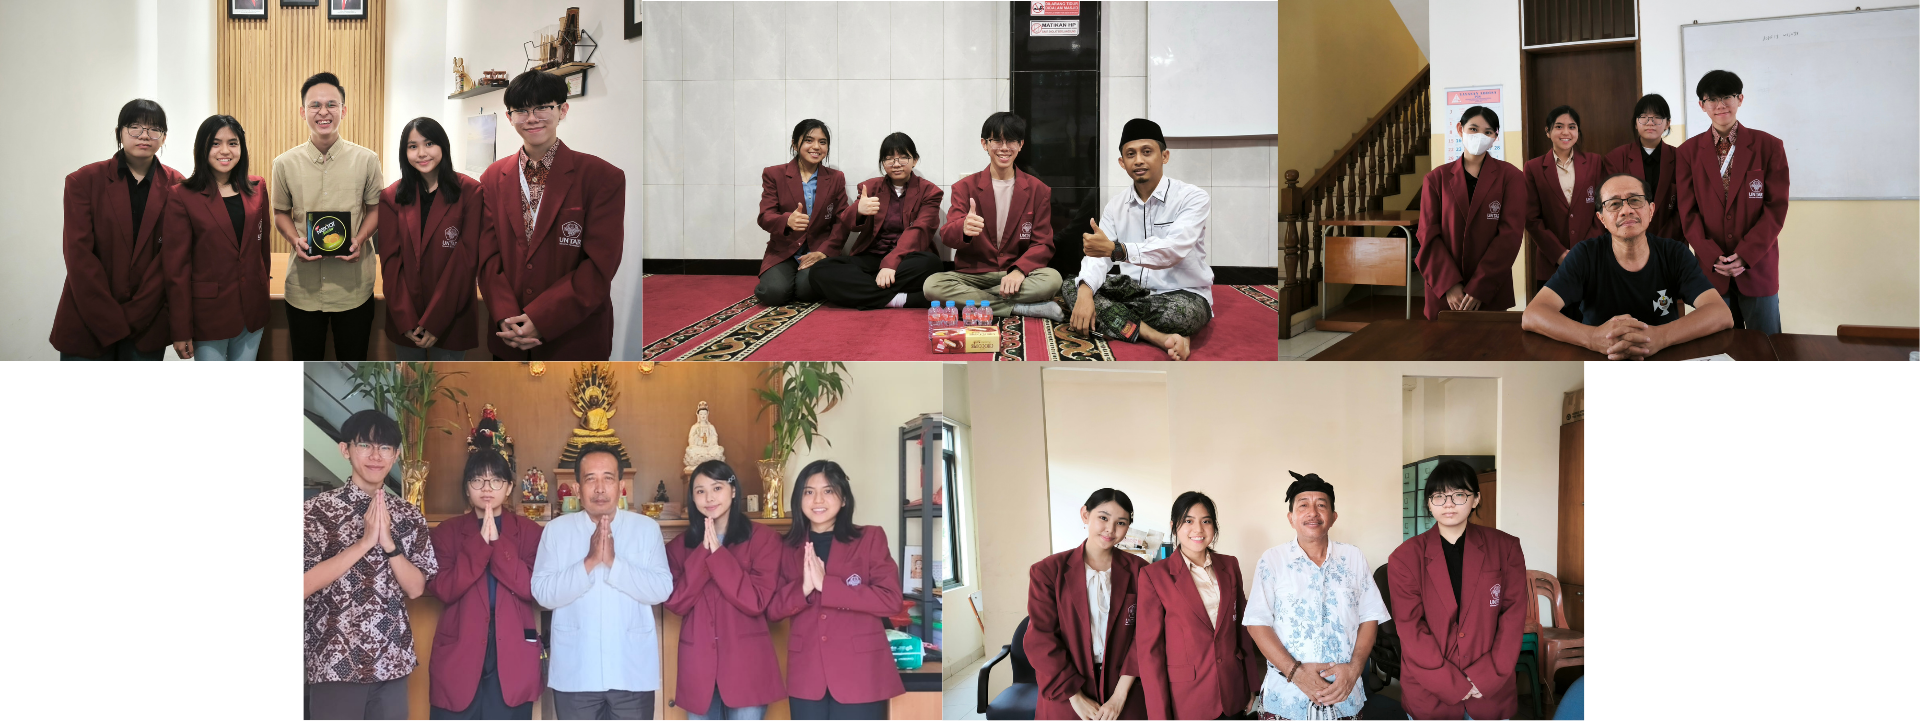
\includegraphics[width=10cm]{assets/documentation/foto_narasumber_all.png}
              \captionsetup{labelformat=empty}
               \caption[Foto bersama para narasumber]{Gambar \ref{fig:FOTONARASUMBER} Foto bersama para narasumber kegiatan wawancara}
            \label{fig:FOTONARASUMBER}
        \end{figure}

Dokumentasi kegiatan menunjukkan pelaksanaan wawancara bersama para narasumber dari berbagai latar belakang agama. Foto bersama narasumber menjadi bukti bahwa kegiatan studi lapangan telah dilaksanakan secara langsung. Melalui kegiatan wawancara ini, tim peneliti memperoleh pemahaman yang lebih luas mengenai bagaimana masing-masing agama memandang tindakan korupsi dan bagaimana nilai keagamaan dapat digunakan untuk menanamkan moral antikorupsi kepada masyarakat.
    
Kegiatan wawancara juga memperlihatkan bahwa isu korupsi tidak hanya dapat dibahas dari sudut pandang hukum, tetapi juga dari sudut pandang moral dan spiritual. Setiap narasumber memberikan penekanan yang berbeda sesuai dengan ajaran agamanya, namun seluruhnya sepakat bahwa korupsi merupakan tindakan yang merusak nilai kejujuran, tanggung jawab, dan keadilan sosial. Oleh karena itu, dokumentasi kegiatan ini menjadi bagian penting dalam laporan karena menunjukkan keterlibatan langsung narasumber dalam memberikan perspektif keagamaan terhadap moral antikorupsi.
